19. \begin{figure}[ht!]
\center{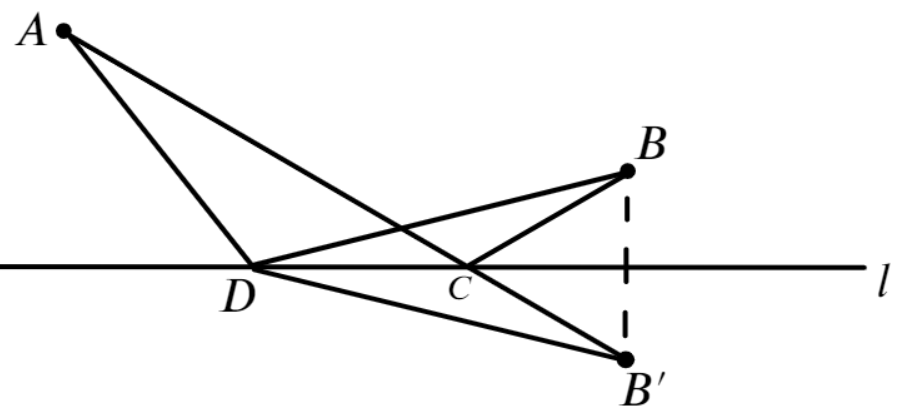
\includegraphics[scale=0.35]{g8-19.png}}
\end{figure}\\
Отразим точку $B$ симметрично относительно прямой $l,$ получим точку $B'.$ Пусть прямая $AB'$ пересекает прямую $l$ в точке $C.$ Докажем, что именно эта точка будет искомой. Возьмём на прямой $l$ другую точку $D.$ Тогда $AC+BC=AC+B'C=AB'<AD+B'D\text{ (по неравенству треугольника) }=AD+BD.$\\
